\documentclass[conference]{IEEEtran}
\IEEEoverridecommandlockouts
% The preceding line is only needed to identify funding in the first footnote. If that is unneeded, please comment it out.
\usepackage{cite}
\usepackage{amsmath,amssymb,amsfonts}
% \usepackage{algorithm,algorithmic}
\usepackage[ruled,vlined]{algorithm2e}
\usepackage{graphicx}
\usepackage{textcomp}
\usepackage{booktabs}
\usepackage[table,xcdraw]{xcolor}
\graphicspath{{../images/}}
\def\BibTeX{{\rm B\kern-.05em{\sc i\kern-.025em b}\kern-.08em
    T\kern-.1667em\lower.7ex\hbox{E}\kern-.125emX}}
\begin{document}

\title{Evolving Simple Models for Regression, Classification, and Clustering}

\author{\IEEEauthorblockN{Evan Lavender}
\IEEEauthorblockA{edl43@drexel.edu}}

\maketitle

\begin{abstract}
This paper presents the use of evolutionary black-box optimization techniques to perform supervised linear and binary logistic regression 
and unsupervised data clustering. The algorithms used are a naive \emph{Evolution Strategy} (ES), a \emph{genetic algorithm} variant of ES, 
a \emph{Natural Evolution Strategy} (NES), and \emph{Differential Evolution} (DE). The \texttt{LinearRegression}, \texttt{LogisticRegression}, 
and \texttt{KMeans} models implemented by \cite{scikit} are used for comparison. Toy data is generated by \cite{scikit} and used to demonstrate 
regression, classification, and clustering. Real data from \cite{molecules}\footnote{https://www.kaggle.com/burakhmmtgl/energy-molecule} is used 
for regression, and real data from \cite{pulsar}\footnote{https://www.kaggle.com/pavanraj159/predicting-a-pulsar-star} is used for binary 
classification. The experiments show metrics comparable to, and sometimes slightly better than the traditional techniques for linear and logistic 
regression and clustering.
\end{abstract}

\begin{IEEEkeywords}
evolutionary algorithm, evolution strategy, natural evolution strategy, differential evolution, black-box optimization
\end{IEEEkeywords}

\section{Introduction}
Evolution Strategy and Differential Evolution algorithms belong to the \emph{evolutionary algorithm} family. Both belong to the class of black 
box optimization algorithms that are heuristic search procedures inspired by natural evolution: At every iteration, a population of 
parameter vectors is perturbed and their objective function is evaluated \cite{openai}. The highest scoring (\emph{fitness}) parameter vectors are then 
recombined to form the population for the next generation \cite{openai}. This procedure is repeated until the objective function is 
optimized \cite{openai}. The two types of algorithms differ in how they perform the perturbation (\emph{mutation}) and recombination.

Black-box optimization algorithms are meant to operate on optimization problems that too difficult or complex to model directly. When the objective 
function is nonlinear and non-differentiable, direct search approaches are the methods of choice \cite{de}. The objective function can be treated as 
a \emph{black-box}; requiring no additional information besides fitness evaluations at certains points in parameter space \cite{nes}. This can be seen 
as estimating the gradient of the objective function by using the finite differences between solutions in the population.

The ES and DE algorithms differ in when they create the population, how they sample the solutions, and how they update parameters. 
ES algorithms typically create a population at the beginning of each iteration by sampling a normal distribution. The $\mu$ parameter of the 
distribution represents the best or \emph{mean} solution found so far. The $\sigma$ parameter may either be fixed, or updated during iteration. This 
random sampling serves to generate \emph{mutations} of the best ($\mu$) solution found. The DE algorithm has a hyperparameter of \emph{bounds}, 
which are used to sample an initial population from a uniform distribution. This population is then evolved in place, with mutated solutions 
created using the difference between other solutions. 

\section{Related Work}
The problem of black-box optimization has spawned a wide variety of approaches \cite{nes}. In addition to evolution strategies and differential 
evolution algorithms, these include the broad class of genetic algorithms, simulated annealing \cite{sim}, particle swarm optimization \cite{part}, 
and others. Evolution strategies were designed to cope with high-dimensional continuous-valued domains and have remained an active field of research 
for more than four decades \cite{es}. 

The naive ES variant is described in \cite{otoro}. This implementation is very greedy in nature, and throws away all but the single best solution. 
The genetic algorithm variant is also described in \cite{otoro}. The idea is to keep a percentage of the best solutions, and sample the new population 
from them. \cite{openai} describes a natural evolution strategy. NES algorithms maximize the average objective value over the \emph{entire} population.

\cite{de} introduces the differential evolution algorithm. DE generates new solutions by adding a weighted difference vector between two solutions to 
a third solution \cite{de}. For each member of the population, a potential solution is generated and will replace the current member if it has a 
higher objective fitness value.

\section{Methodology}
\subsection{Simple/Naive Evolution Strategy}
The simplest evolution strategy samples from a normal distribution with a mean $\mu$ and a fixed standard deviation $\sigma$ \cite{otoro}. After the 
fitness results are evaluated, $\mu$ is set to the best solution in the population \cite{otoro}. The next generation of samples is then centered around 
this new mean. The initial value for $\mu$ is a zero-vector.

\begin{algorithm}[htbp]
\SetAlgoLined
\KwIn{standard deviation $\sigma$}
    \For{$g = 0, 1, 2, ...$}{
        Sample $x_i, ..., x_n \sim \mathcal{N}(\mu_g, \sigma) \sim \mu_g + \sigma\mathcal{N}(0, I)$ \\
        Compute returns $F_i = F(x_i)$ for $i = 1, ..., n$ \\
        Set $\mu_{g+1} = \max{F_i}$ \\
    }
\caption{Naive Evolution Strategy}
\label{alg:ses}
\end{algorithm}

\subsection{Simple Genetic Algorithm}
Instead of only selecting the best solution, the genetic algorithm implementation will keep a percentage of the best solutions. Sampling a new solution 
involves adding Gaussian noise to a solution that is created by combining two solutions from the previous generation. For each solution in the 
population, two solutions of the previous generation are randomly selected to be combined. The recombination process takes a parameter from either 
solution with a $50$\% chance. Finally, this new solution has the sampled noise added to it.

\begin{algorithm}[htbp]
\SetAlgoLined
\KwIn{standard deviation $\sigma$, number of parents $\lambda$}
    Initialize parents $p_g = p_i, ..., p_\lambda$ \\
    \For{$g = 0, 1, 2, ...$}{
        Sample $x_i, ..., x_n \sim \mathcal{N}(0, \sigma) \sim \sigma\mathcal{N}(0, I)$ \\
        Recombine $\lambda$ parents, add to $x_i, ..., x_n$ \\
        Compute returns $F_i = F(x_i)$ for $i = 1, ..., n$ \\
        Set $p_{g+1} = \max_{1...\lambda}{F}$ \\
        Set $\mu_{g+1} = \frac{1}{\lambda}\sum{p_{g+1}}$ \\
    }
\caption{Genetic Evolution Strategy}
\label{alg:ges}
\end{algorithm}

\subsection{Natural Evolution Strategy}
The natural evolution strategy algorithm described in \cite{openai} is very similar to the naive variation; they differ only in how the parameters 
are updated. This NES algorithm takes every member of the population into account when updating the $\mu$ parameter for the distribution.

\begin{algorithm}[htbp]
\SetAlgoLined
\KwIn{standard deviation $\sigma$, learning rate $\alpha$}
    \For{$g = 0, 1, 2, ...$}{
        Sample $\epsilon_i, ..., \epsilon_n \sim \mathcal{N}(0, I)$ \\
        Compute returns $F_i = F(\mu_g + \sigma\epsilon_i)$ for $i = 1, ..., n$ \\
        Set $\mu_{g+1} = \mu_g + \alpha \frac{1}{n\sigma} \sum_{i=1}^n{F_i\epsilon_i}$ \\
    }
\caption{Natural Evolution Strategy}
\label{alg:nes}
\end{algorithm} \cite{openai}

\subsection{Differential Evolution}
The Differential Evolution algorithm is not a variation of an evolution strategy, but is still within the family of evolutionary algorithms. 
An initial population is sampled from a uniform distribution with bounds set as a hyperparameter for the algorithm. The crucial idea behind DE 
is a scheme for generating trial parameter vectors \cite{de}. DE generates new parameter vectors by adding a weighted difference (\emph{differential}) 
vector between two population members for a third member \cite{de}. This resulting vector is evaulated, and if its value is greater than the value of 
a predetermined population member, then it will replace that member for the following generation \cite{de}. 

Trial vectors are generated according to
$$
    v = x + \lambda (x_{best} - x) + F (x_2 - x_3)
$$
where $x_2$ and $x_3$ are randomly selected and $\neq x$, and $F > 0$ \cite{de}. $F$ is a parameter for controlling the amplification of 
the differential variation \cite{de}. $\lambda$ provides a means to enhance greediness by incorporating the current best solution $x_{best}$ \cite{de}.

The final trial vector is created by setting each parameter to either $v_i$ or $x_i$ for $i = 1, ..., n$, according to a crossover probability 
hyperparameter. If the value of this new vector is greater than the value of $x$, $x$ will be replaced with $v$.

\begin{algorithm}[htbp]
\SetAlgoLined
\KwIn{bounds $b_{min}, b_{max}$, parameter $F$, parameter $\lambda$}
    Initial population $x = \mathcal{U}(b_{min}, b_{max})$ \\
    Set $x_{best} = \max{F(x)}$ \\
    \For{$g = 0, 1, 2, ...$}{
        \For{$x_i$ in $i = 1, ..., n$}{
            Sample vectors $x_2, x_3 = choice(x) \neq x_i$ \\
            Create trial vector $v = x_i + \lambda (x_{best} - x_i) + F (x_2 - x_3)$ \\
            Set $v_i = v_i$ if $rand() < p_{cx} $ else $x_i$ \\
            Replace $x_i$ if $F(v) > F(x_i)$ \\
        }
        Set $x_{best} = \max{F(x)}$
    }
\caption{Differential Evolution}
\label{alg:dev}
\end{algorithm}

\subsection{Objective Functions}
\subsubsection{Regression}
The objective function for the regression models is the residual sum of squares between the observed targets in the dataset, and the targets 
predicted by the model \cite{scikit}. The algorithm will maximize the negative of this value; minimizing the function.
$$
    \lVert X\mu - y \rVert_{2}^{2}
$$

\subsubsection{Classification}
The objective function for the binary classification models is the cross entropy function. The predictions are first passed through a sigmoid function. 
The algorithm will maximize this value.
$$
    \sum_{i=1}^{N}{y \log{X\mu} + (1 - y)\log{1 - X\mu}}
$$

\subsubsection{Clustering}
The objective function for the clustering models will compute the inertia value of the reference vectors. The algorithm will maximize the negative of 
this value; minimizing the function.

\section{Experiments and Results}
\subsection{Regression}
\subsubsection{Toy Problems}
Each of the four algorithms was used to evolve a linear regression model of data created using \cite{scikit}'s \texttt{make\_regression} function. 
The data consists of $2500$ samples with $100$ features. The data is split into training and testing sets with a \texttt{test\_size} of $0.3$. The 
regression metrics calculated are $R^2$ score, explained variance score, and root-mean-square error (RMSE). A \texttt{LinearRegression} model from 
\cite{scikit} is trained on the same data for comparison (see Table \ref{tab:toy-regr1}). Finally, cross-validation is performed on all five models to 
get a final $R^2$ score for each (see Table \ref{tab:toy-regr2}). See Fig. \ref{plot:toy-score} in the appendix for plots of the model score curves.

\begin{table}[htbp]
\centering
\begin{tabular}{@{}llll@{}}
\toprule
 & R2 Score & Explained Variance Score & RMSE \\ \midrule
Linear Regression & 0.93038 & 0.93067 & 104.26580 \\
Simple ES & 0.92989 & 0.93018 & 104.62999 \\
Genetic ES & 0.92876 & 0.92899 & 105.47040 \\
Natural ES & \cellcolor[HTML]{C0C0C0}0.93054 & \cellcolor[HTML]{C0C0C0}0.93083 & \cellcolor[HTML]{C0C0C0}104.14309 \\
DE & 0.92932 & 0.92969 & 105.05684 \\ \bottomrule
\end{tabular}
\caption{Toy regression metrics}
\label{tab:toy-regr1}
\end{table}

\begin{table}[htbp]
\centering
\begin{tabular}{@{}ll@{}}
\toprule
 & Cross Validated R2 Score \\ \midrule
Linear Regression & 0.93710 (+/- 0.00627) \\
Simple ES & 0.93438 (+/- 0.00435) \\
Genetic ES & 0.93192 (+/- 0.00824) \\
Natural ES & 0.93710 (+/- 0.00634) \\
DE & 0.93535 (+/- 0.00774) \\ \bottomrule
\end{tabular}
\caption{Toy regression metrics}
\label{tab:toy-regr2}
\end{table}

We can see from the results that the models are all fairly close in performance with this data. Due to the inherent randomness of the evolutionary 
algorithms, they may produce a different set of parameters with a different random seed. The NES model may have outperformed standard Linear 
Regression after one trial, but we should not make conclusions from that alone. \cite{scikit}'s \texttt{cross\_val\_score} was used to perform 
cross-validation. We see NES and Linear Regression have almost equal performance, and the other are slightly behind.

\subsubsection{Ground State Energies of 16242 Molecules}
Each model was tested on a real world dataset consisting of the ground state energies of $16242$ molecules calculated by quantum mechanical 
simulations \cite{molecules}. There are $1275$ columns used that act as molecular features, with the final column being the atomization energy as 
calulated by simulate \cite{molecules}. The inspiration behind this dataset stems from the problem that simulations of molecular properties are 
computationally expensive \cite{molecules}. Being able to use a model to predict molecular properties could open up many possibilities in 
computational design and discovery of molecules, compounds and new drugs \cite{molecules}.

Initial results with \texttt{LinearRegression} gave an overfitted model with a $R^2$ score of $-3685.75153$. Using principal component analysis (PCA), 
it was determined that 50 components gave an acceptable amount of explained variance of $0.99448$ (see Fig. \ref{fig:exp}). Kernel PCA (kPCA) was 
performed in addition to standard PCA for feature reduction. kPCA resulted in more variance being captured in the same number of components, so it was 
used for the final results. The first $16$ components and their relation to the energy levels for both PCA and kPCA can be seen in Figures \ref{fig:pca} 
and \ref{fig:kpca} in the appendix.
\begin{figure}[htbp]
\centering
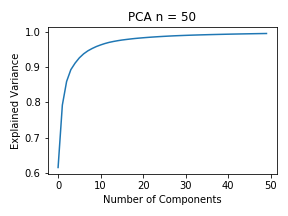
\includegraphics[width=.4\textwidth]{Molecules-ExplainedVariance.png}
\caption{Molecules - Explained Variance}
\label{fig:exp}
\end{figure}

The trials remain the same from the toy example. Metrics can be seen in tables \ref{tab:mol-regr1} and \ref{tab:mol-regr2}. Score curves can be seen 
in Figure \ref{plot:mol-score} in the appendix. The Differential Evolution model slightly outperformed Linear Regression after cross-validation.

\begin{table}[htbp]
\centering
\begin{tabular}{@{}llll@{}}
\toprule
 & R2 Score & Explained Variance Score & RMSE \\ \midrule
Linear Regression & \cellcolor[HTML]{C0C0C0}0.97600 & \cellcolor[HTML]{C0C0C0}0.97601 & \cellcolor[HTML]{C0C0C0}0.56078 \\
Simple ES & 0.97305 & 0.97311 & 0.59432 \\
Genetic ES & 0.96871 & 0.96872 & 0.64042 \\
Natural ES & 0.94426 & 0.94866 & 0.85473 \\
DE & \cellcolor[HTML]{C0C0C0}0.97600 & 0.97600 & 0.56087 \\ \bottomrule
\end{tabular}
\caption{Molecule regression metrics}
\label{tab:mol-regr1}
\end{table}

\begin{table}[htbp]
\centering
\begin{tabular}{@{}ll@{}}
\toprule
 & Cross Validated R2 Score \\ \midrule
Linear Regression & 0.97651 (+/- 0.01405) \\
Simple ES & 0.97382 (+/- 0.01514) \\
Genetic ES & 0.96069 (+/- 0.01815) \\
Natural ES & 0.93126 (+/- 0.03337) \\
DE & 0.97654 (+/- 0.01404) \\ \bottomrule
\end{tabular}
\caption{Molecule regression metrics}
\label{tab:mol-regr2}
\end{table}

\subsection{Classification}
\subsubsection{Toy Problems}
Each of the four algorithms was used to evolve a linear classification model of data created using \cite{scikit}'s \texttt{make\_classification} function. 
The data consists of $2500$ samples with $100$ features. The data is split into training and testing sets with a \texttt{test\_size} of $0.3$. A 
classification report and PR curve are generated for each model. A \texttt{LogisticRegression} model from \cite{scikit} is trained on the same data 
for comparison (see Table \ref{tab:toy-class1}). Finally, cross-validation is performed on all five models to get a final accuracy score for each 
(see Table \ref{tab:toy-class2}). See Fig. \ref{plot:toy-pr} in the appendix for plots of the model PR curves.

\begin{table}[htbp]
\centering
\begin{tabular}{@{}lllll@{}}
\toprule
 & Precision & Recall & F1-Score & Accuracy \\ \midrule
Logistic Regression & \cellcolor[HTML]{C0C0C0}0.96 & \cellcolor[HTML]{C0C0C0}0.96 & \cellcolor[HTML]{C0C0C0}0.96 & \cellcolor[HTML]{C0C0C0}0.96 \\
Simple ES & 0.94 & 0.94 & 0.94 & 0.94 \\
Genetic ES & 0.92 & 0.92 & 0.92 & 0.92 \\
Natural ES & 0.94 & 0.94 & 0.94 & 0.94 \\
DE & 0.89 & 0.89 & 0.89 & 0.89 \\ \bottomrule
\end{tabular}
\caption{Toy classification metrics}
\label{tab:toy-class1}
\end{table}

\begin{table}[htbp]
\centering
\begin{tabular}{ll}
\hline
 & Cross-Validated Accuracy \\ \hline
Logistic Regression & 0.96080 (+/- 0.01229) \\
Simple ES & 0.93000 (+/- 0.02400) \\
Genetic ES & 0.93560 (+/- 0.00993) \\
Natural ES & 0.95880 (+/- 0.01353) \\
DE & 0.91080 (+/- 0.03825) \\ \hline
\end{tabular}
\caption{Toy classification metrics}
\label{tab:toy-class2}
\end{table}

We can see that standard Logistic Regression has better performance on this dataset.

\subsubsection{Predicting a Pulsar Star}
The HTRU2 is a dataset which describes a sample of pulsar candidates collected during the High Time Resolution Universe Survey \cite{pulsar}. 
Pulsars are a rare type of Neutron start that produce radio emission detectable here on Earth \cite{pulsar}. They are of considerable scientific 
interest as probes of space-time, the interstellar medium, and states of matter \cite{pulsar}. Each candidate is described by $8$ continuous 
variables and a single binary class variable \cite{pulsar}. The experiments are the same as the toy problem; metrics can be seen in tables 
\ref{tab:pul-class1} and \ref{tab:pul-class2}, and PR curves can be seen in Figure \ref{plot:pul-pr} in the appendix.

\begin{table}[htbp]
\centering
\begin{tabular}{@{}lllll@{}}
\toprule
 & Precision & Recall & F1-Score & Accuracy \\ \midrule
Logistic Regression & \cellcolor[HTML]{C0C0C0}0.96 & 0.91 & 0.93 & \cellcolor[HTML]{C0C0C0}0.98 \\
Simple ES & \cellcolor[HTML]{C0C0C0}0.96 & \cellcolor[HTML]{C0C0C0}0.92 & \cellcolor[HTML]{C0C0C0}0.94 & \cellcolor[HTML]{C0C0C0}0.98 \\
Genetic ES & \cellcolor[HTML]{C0C0C0}0.96 & 0.90 & 0.93 & \cellcolor[HTML]{C0C0C0}0.98 \\
Natural ES & \cellcolor[HTML]{C0C0C0}0.96 & 0.90 & 0.93 & \cellcolor[HTML]{C0C0C0}0.98 \\
DE & \cellcolor[HTML]{C0C0C0}0.96 & 0.91 & 0.93 & \cellcolor[HTML]{C0C0C0}0.98 \\ \bottomrule
\end{tabular}
\caption{Pulsar classification metrics}
\label{tab:pul-class1}
\end{table}

\begin{table}[htbp]
\centering
\begin{tabular}{ll}
\hline
 & Cross-Validated Accuracy \\ \hline
Logistic Regression & 0.97810 (+/- 0.00488) \\
Simple ES & 0.97838 (+/- 0.00639) \\
Genetic ES & 0.97709 (+/- 0.00469) \\
Natural ES & 0.97620 (+/- 0.00546) \\
DE & 0.97888 (+/- 0.00440) \\ \hline
\end{tabular}
\caption{Pulsar classification metrics}
\label{tab:pul-class2}
\end{table}

The pulsar dataset is unbalanced; with 16259 negative samples and 1639 negative samples. The single trials give every model equal precision and 
accuracy, but differing recall and F1-scores. The simle ES model found parameters that slightly outperformed Logistic Regression in recall and 
F1-score, with equal precision and accuracy. After cross-validation, the simple ES and DE models both have higher accuracy than Logistic Regression, 
with DE on top.

\subsection{Clustering}
Each of the four algorithms was used to evolve a set of reference vectors that cluster the data created using \cite{scikit}'s \texttt{make\_blobs} 
function. The data consists of $250$ samples with $2$ features and $10$ clusters. Homogeneity, completeness, v-measure, and inertia are computed 
for each model, and scores are graphed (see Figure \ref{plot:toy-clus} in the appendix). A \texttt{KMeans} model from \cite{scikit} is used on the same 
data for comparison (see Table \ref{tab:toy-clus}). The clusters can be seen in Figure \ref{plot:clus}.

\begin{figure}[htbp]
\centering
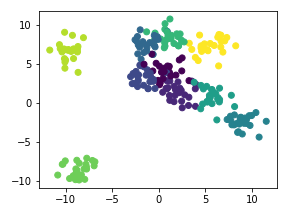
\includegraphics[width=.4\textwidth]{Toy-Clusters.png}
\caption{Clusters}
\label{plot:clus}
\end{figure}

We can see the NES model created clusters with the highest homogeneity, completeness, and V-measure. The DE model has the lowest inertia, or 
within-cluster sum-of-squares. The DE model outperformed k-means in every metric computed with this dataset. An interesting thing to notice is that 
the simple ES model created a cluster that has nothing assigned to it. There were no constraints against this in the objective function, so the 
algorithm got stuck in a local optimum that includes that empty cluster.

\begin{table}[htbp]
\centering
\begin{tabular}{@{}lllll@{}}
\toprule
 & Homogeneity & Completeness & V-Measure & Inertia \\ \midrule
K-Means & 0.88091 & 0.88220 & 0.88156 & 432.20263 \\
Simple ES & 0.84160 & 0.89568 & 0.86780 & 539.64422 \\
Genetic ES & 0.85756 & 0.86349 & 0.86051 & 506.09878 \\
Natural ES & \cellcolor[HTML]{C0C0C0}0.90360 & \cellcolor[HTML]{C0C0C0}0.90441 & \cellcolor[HTML]{C0C0C0}0.90401 & 448.04099 \\
DE & 0.89660 & 0.89728 & 0.89694 & \cellcolor[HTML]{C0C0C0}431.09699 \\ \bottomrule
\end{tabular}
\caption{Toy clustering metrics}
\label{tab:toy-clus}
\end{table}

\section{Conclusions}
Two evolutionary optimization techniques were introduced: Evolution Strategies and Differential Evolution. Three variations of the 
Evolution Strategy technique were used: simple/naive ES, a genetic algorithm ES, and a natural ES. Normally used for black-box optimization, the 
algorithms were instead trialed against traditional regression, classification, and clustering techniques; namely linear regression, logistic 
regression, and k-means clustering. Experiments were ran on toy data generated by \cite{scikit}, and real datasets from \cite{molecules} and 
\cite{pulsar}. The models generated were shown to have acceptable performance in most cases, and superior performance in others. 

\section{Future Work}
There is a large amount of future work that could improve upon these algorithms, and there are many variations on the evolution strategy that 
could be implemented. Hyperparameter optimization could be performed to fine-tune each model for a particular dataset. The effect each parameter has 
on the performance of the algorithm was not explored deeply.

An important property for an optimizer is to guarantee finding the global optimum. This constraint was not satisfied in thie work, as the algorithms 
would reliably settle in a local optimum. Many objective functions exist for the tasks of regression, classification, and clustering. 
This work only presented a single one for each. 

Rather than evolving models directly, evolutionary algorithms are commonly used to evolve neural network parameters. \cite{openai} explored Evolution 
Strategies as an alternative to popular reinforcement-learning techniques. There are many interesting problems that can be explored. 

\bibliographystyle{ieeetr}
\bibliography{refs}

\appendix

\begin{figure*}[htbp]
\centering
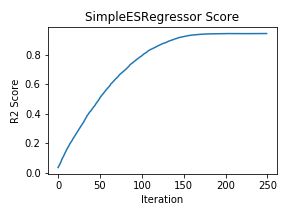
\includegraphics[width=.4\textwidth]{Toy-SimpleESRegressor-ScoreCurve.png}
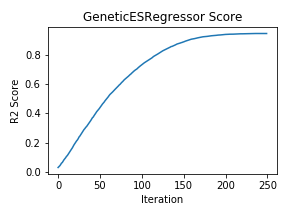
\includegraphics[width=.4\textwidth]{Toy-GeneticESRegressor-ScoreCurve.png}
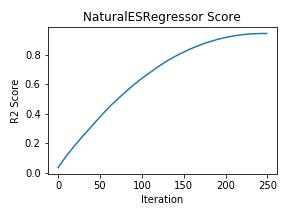
\includegraphics[width=.4\textwidth]{Toy-NaturalESRegressor-ScoreCurve.png}
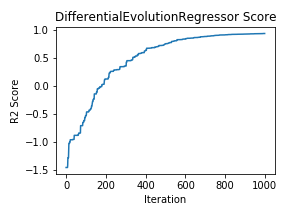
\includegraphics[width=.4\textwidth]{Toy-DifferentialEvolutionRegressor-ScoreCurve.png}
\caption{Toy regression model score curves}
\label{plot:toy-score}
\end{figure*}

\begin{figure*}[htbp]
\centering
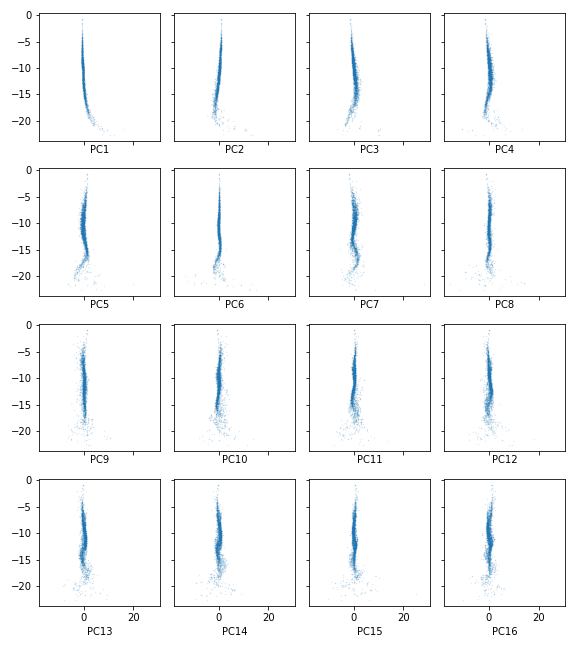
\includegraphics[width=\textwidth]{Molecules-PCA.png}
\caption{Molecules - PCA}
\label{fig:pca}
\end{figure*}

\begin{figure*}[htbp]
\centering
\includegraphics[width=\textwidth]{Molecules-kPCA.png}
\caption{Molecules - kPCA}
\label{fig:kpca}
\end{figure*}

\begin{figure*}[htbp]
\centering
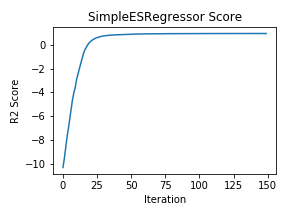
\includegraphics[width=.4\textwidth]{Molecules-SimpleESRegressor-kPCAScoreCurve.png}
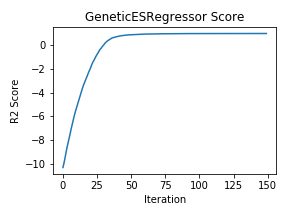
\includegraphics[width=.4\textwidth]{Molecules-GeneticESRegressor-kPCAScoreCurve.png}
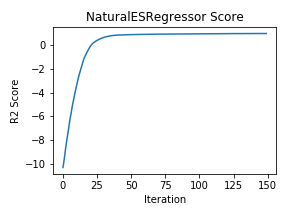
\includegraphics[width=.4\textwidth]{Molecules-NaturalESRegressor-kPCAScoreCurve.png}
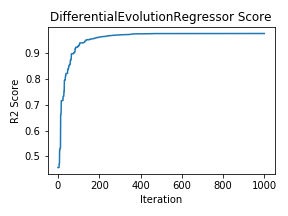
\includegraphics[width=.4\textwidth]{Molecules-DifferentialEvolutionRegressor-kPCAScoreCurve.png}
\caption{Molecule regression model score curves}
\label{plot:mol-score}
\end{figure*}

\begin{figure*}[htbp]
\centering
\makebox[\textwidth][c]{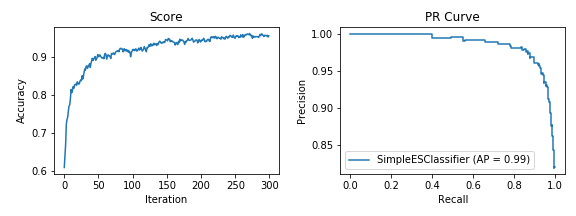
\includegraphics[height=.25\textheight,keepaspectratio]{Toy-SimpleESClassifier-PRCurve.png}}
\makebox[\textwidth][c]{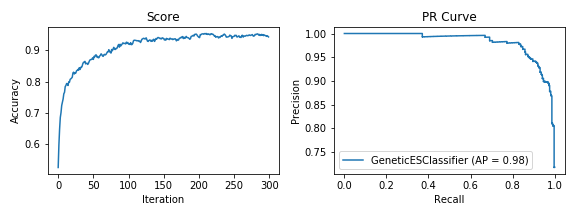
\includegraphics[height=.25\textheight,keepaspectratio]{Toy-GeneticESClassifier-PRCurve.png}}
\makebox[\textwidth][c]{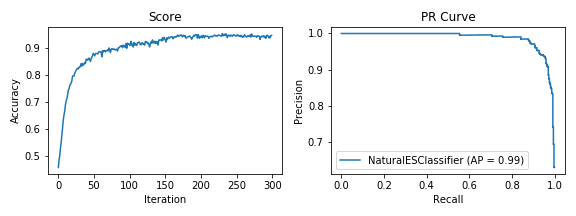
\includegraphics[height=.25\textheight,keepaspectratio]{Toy-NaturalESClassifier-PRCurve.png}}
\makebox[\textwidth][c]{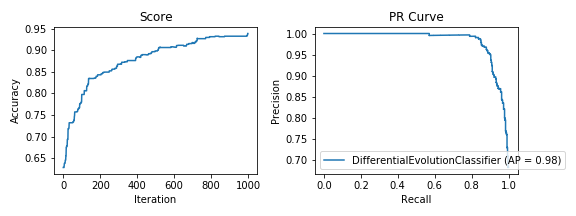
\includegraphics[height=.25\textheight,keepaspectratio]{Toy-DifferentialEvolutionClassifier-PRCurve.png}}
\caption{Toy classification model score curves}
\label{plot:toy-pr}
\end{figure*}

\begin{figure*}[htbp]
\centering
\makebox[\textwidth][c]{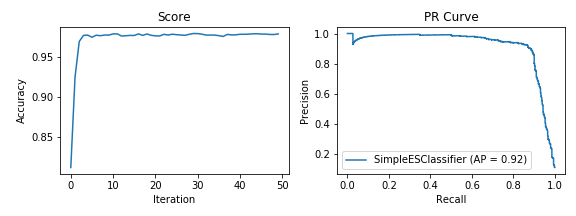
\includegraphics[height=.25\textheight,keepaspectratio]{Pulsar-SimpleESClassifier-PRCurve.png}}
\makebox[\textwidth][c]{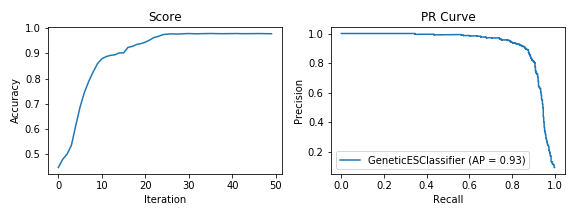
\includegraphics[height=.25\textheight,keepaspectratio]{Pulsar-GeneticESClassifier-PRCurve.png}}
\makebox[\textwidth][c]{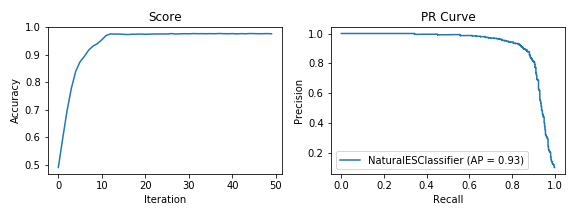
\includegraphics[height=.25\textheight,keepaspectratio]{Pulsar-NaturalESClassifier-PRCurve.png}}
\makebox[\textwidth][c]{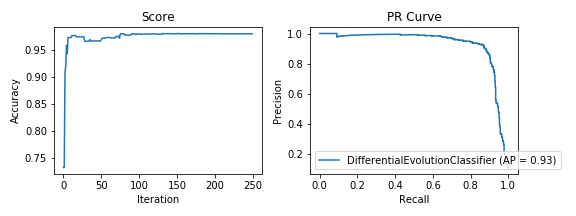
\includegraphics[height=.25\textheight,keepaspectratio]{Pulsar-DifferentialEvolutionClassifier-PRCurve.png}}
\caption{Pulsar classification model score curves}
\label{plot:pul-pr}
\end{figure*}

\begin{figure*}[htbp]
\centering
\makebox[\textwidth][c]{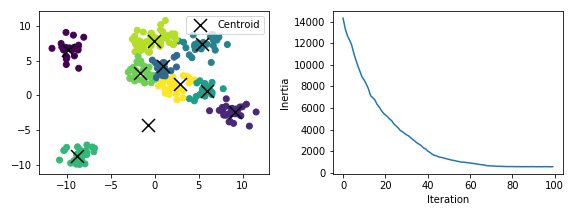
\includegraphics[height=.25\textheight,keepaspectratio]{Toy-SimpleESClustering-Clusters.png}}
\makebox[\textwidth][c]{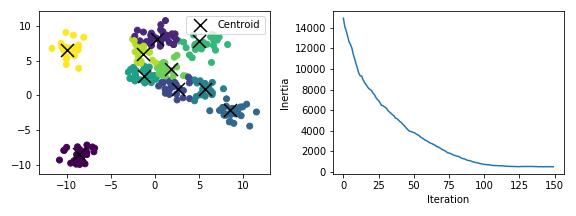
\includegraphics[height=.25\textheight,keepaspectratio]{Toy-GeneticESClustering-Clusters.png}}
\makebox[\textwidth][c]{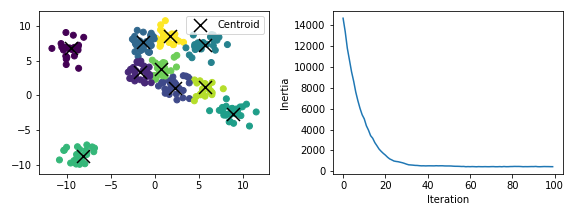
\includegraphics[height=.25\textheight,keepaspectratio]{Toy-NaturalESClustering-Clusters.png}}
\makebox[\textwidth][c]{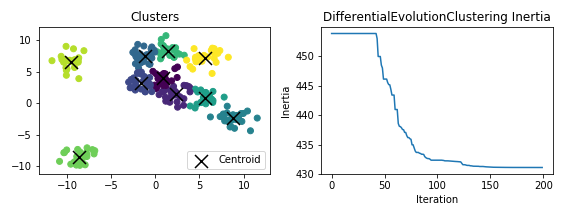
\includegraphics[height=.25\textheight,keepaspectratio]{Toy-DifferentialEvolutionClustering-Clusters.png}}
\caption{Toy clustering}
\label{plot:toy-clus}
\end{figure*}

\end{document}
